%%%%%%%%%%%%%%%%%%%%%%%%%%%%%%%%%%%%%%%%%
% University/School Laboratory Report
% LaTeX Template
% Version 3.1 (25/3/14)
%
% This template has been downloaded from:
% http://www.LaTeXTemplates.com
%
% Original author:
% Linux and Unix Users Group at Virginia Tech Wiki 
% (https://vtluug.org/wiki/Example_LaTeX_chem_lab_report)
%
% License:
% CC BY-NC-SA 3.0 (http://creativecommons.org/licenses/by-nc-sa/3.0/)
%
%%%%%%%%%%%%%%%%%%%%%%%%%%%%%%%%%%%%%%%%%

%----------------------------------------------------------------------------------------
%	PACKAGES AND DOCUMENT CONFIGURATIONS
%----------------------------------------------------------------------------------------

\documentclass{article}

\usepackage[version=3]{mhchem} % Package for chemical equation typesetting
\usepackage{siunitx} % Provides the \SI{}{} and \si{} command for typesetting SI units
\usepackage{graphicx} % Required for the inclusion of images
\usepackage{natbib} % Required to change bibliography style to APA
\usepackage{amsmath} % Required for some math elements 
\usepackage[utf8]{inputenc}

\setlength\parindent{0pt} % Removes all indentation from paragraphs

\renewcommand{\labelenumi}{\alph{enumi}.} % Make numbering in the enumerate environment by letter rather than number (e.g. section 6)

%\usepackage{times} % Uncomment to use the Times New Roman font

%----------------------------------------------------------------------------------------
%	DOCUMENT INFORMATION
%----------------------------------------------------------------------------------------

\title{M\'etodos num\'ericos para la Ciencia e Ingenier\'ia \\ Tarea 3} % Title

\author{Felipe Toledo B. \\ Rut: 17.519.820-2} % Author name

\date{\today} % Date for the report

\begin{document}

\maketitle % Insert the title, author and date

%----------------------------------------------------------------------------------------
%	SECTION 1
%----------------------------------------------------------------------------------------

\section{Problema 1}

\subsection{Introducci\'on y objetivos}

El objetivo de esta experiencia es integrar num\'ericamente la ecuaci\'on diferencial del Oscilador de Van der Pool, implementando el m\'etodo de Runge Kutta de orden 3. La ecuaci\'on original se observa en (\ref{eq:oscilador}), con $k$ una constante el\'astica, $a$ una constante de largo y $mu$ un coeficiente de roce.

\begin{equation}
  \dfrac{d^2x}{dt^2} = - k x - \mu (x^2 - a^2) \dfrac{dx}{dt}
  \label{eq:oscilador}
\end{equation}


\subsection{Metodolog\'ia}
Para simplificar el problema, primero se reduce la ecuaci\'on usando el cambio de variables $ \frac{x}{a} = y $, $\sqrt{k}t = s$. Tras esto se obtiene (\ref{eq:oscilador_reducido}), con $\mu^* = \frac{\mu a^2}{\sqrt{k}}$.

\begin{equation}
 \dfrac{d^2y}{ds^2} = - y - \mu^* (y^2 - 1) \dfrac{dy}{ds} 
 \label{eq:oscilador_reducido} 
\end{equation}
 
Como existe una derivada de primer orden a la derecha de la ecuaci\'on, para poder resolver la EDO usando el m\'etodo de Runge Kutta es necesario expresarla como el siguiente sistema de ecuaciones:

\begin{equation}
\begin{cases}

 \dfrac{dy}{ds} = v\\ \\
 \dfrac{dv}{ds} = -y - \mu^*(y^2 - 1)v

\end{cases} 
\label{eq:sistema_edos}
\end{equation}

Definiendo las funciones $\frac{dy}{ds} = f(v)$ y $\frac{dv}{ds} = g(y,v)$, se pueden calcular los valores de '$y$' y '$v$' para todo '$s$' (coordenada temporal) usando el algoritmo (\ref{eq:sol_runge_kutta_3}).

\begin{equation}
  \begin{array}{l}
    y_{n+1} = y_n + \frac{1}{6}(k_1 + 4 k_2 + k_3) \\ \\
    v_{n+1} = v_n + \frac{1}{6}(l_1 + 4 l_2 + l_3)
  \end{array}
  \label{eq:sol_runge_kutta_3}
\end{equation}

En (\ref{eq:constantes_runge_kutta_3}) se puede observar c\'omo se calcula cada constante $k_i$, $l_i$, donde $h$ es el par\'ametro de paso temporal entre cada punto calculado.

\begin{equation}
  \begin{array}{l}
    k_1 = h f( v_n ) \\
    l_1 = h g( y_n , v_n ) \\ \\
    
    k_2 = h f( v_n + \frac{1}{2} l_1 ) \\
    l_2 = h g( y_n + \frac{1}{2} k_1 , v_n + \frac{1}{2} l_1 ) \\ \\
    
    k_3 = h f( v_n - l_1 - 2 l_2 ) \\
    l_3 = h g( y_n - k_1 - 2 k_2 , v_n - l_1 - 2 l_2 )
    
  \end{array}
  \label{eq:constantes_runge_kutta_3}
\end{equation}

\vspace{0.5cm}
Los m\'etodos descritos se encuentran implementados en la clase \textit{oscilador\_van\_der\_pool.py}.

\subsection{Resultados}

Se realizaron dos resoluciones con par\'ametros iguales pero condiciones iniciales distintas. Tanto los resultados como las figuras pueden obtenerse ejecutando el script \textit{P1.py}. El valor de los par\'ametros es:

\begin{itemize}
  \item $ mu^* = 1.820 $
  \item $h = 10^-4$
  \item $T_{final} = 20\pi$ 
\end{itemize} 

\subsubsection{Caso 1}

En este caso las condiciones iniciales son:

\begin{equation}
\dfrac{dy}{ds} = 0; y = 0.1
\label{eq:cond_inicial_1}  
\end{equation}
\vspace{0.1cm}

Los resultados puede verse en las Figuras 1 y 2.

\begin{figure}[h]
  \centering
  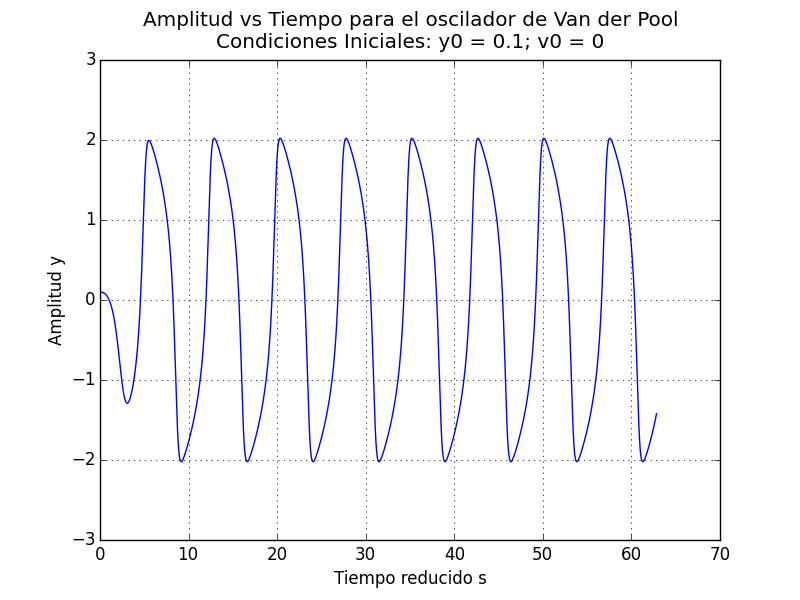
\includegraphics[scale = 0.5]{images/ampl_vs_tiempo_01-0.png}
  \label{}
  \caption{Amplitud vs Tiempo para el oscilador de Van der Pool.}
\end{figure}

\begin{figure}[h]
  \centering
  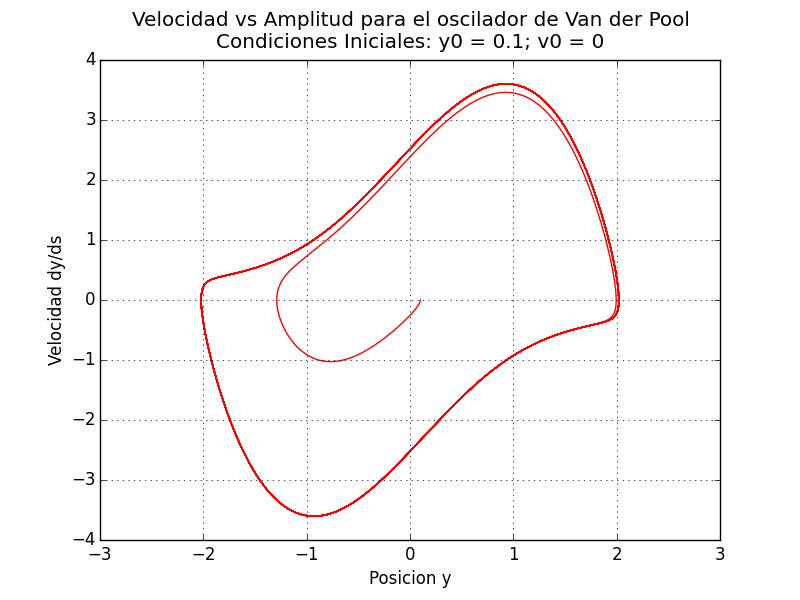
\includegraphics[scale = 0.5]{images/vel_vs_amplitud_01-0.png}
  \label{}
  \caption{Velocidad vs Posici\'on para el oscilador de Van der Pool.}
\end{figure}

\clearpage
\subsubsection{Caso 2}

Los resultados puede verse en las Figuras 3 y 4. Las condiciones iniciales son:

\begin{equation}
\dfrac{dy}{ds} = 0; y = 4.0
\label{eq:cond_inicial_2}  
\end{equation}

\begin{figure}[h]
  \centering
  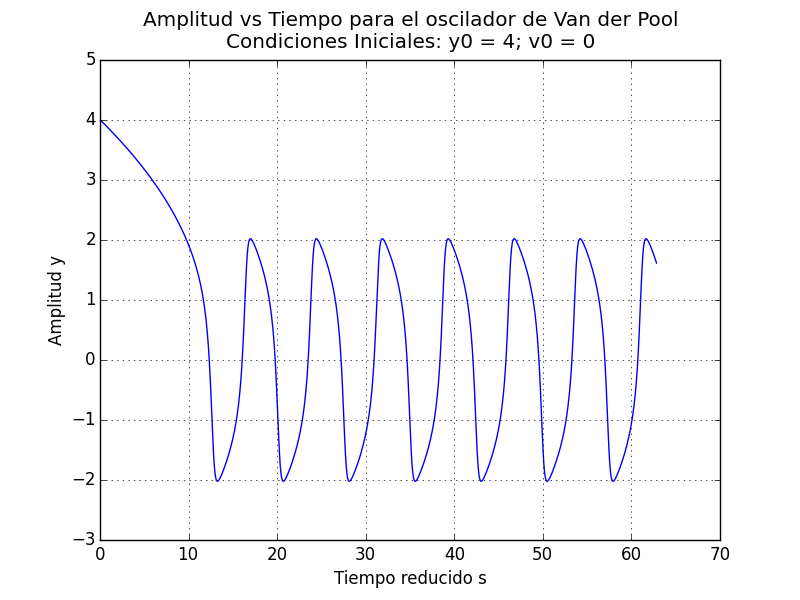
\includegraphics[scale = 0.4]{images/ampl_vs_tiempo_4-0.png}
  \label{}
  \caption{Amplitud vs Tiempo para el oscilador de Van der Pool.}
\end{figure}

\begin{figure}[h]
  \centering
  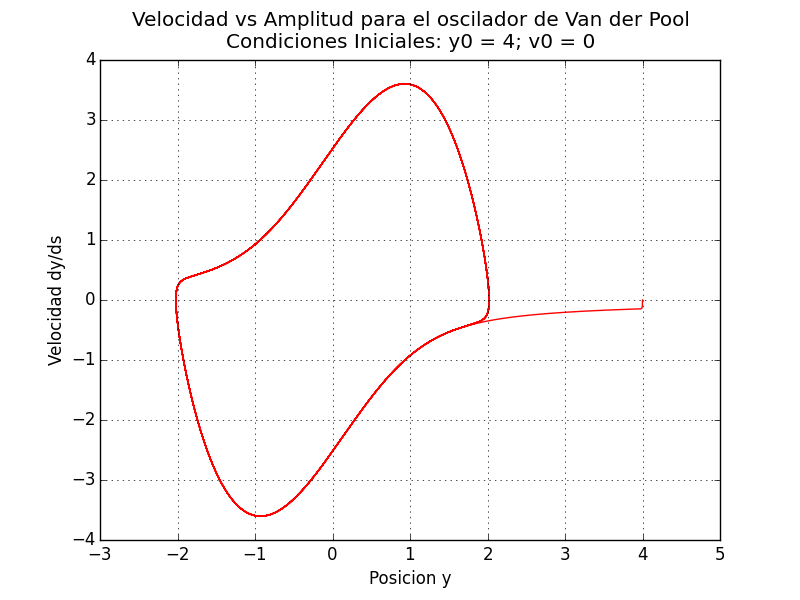
\includegraphics[scale = 0.4]{images/vel_vs_amplitud_4-0.png}
  \label{}
  \caption{Velocidad vs Posici\'on para el oscilador de Van der Pool.}
\end{figure}

 \subsection{Conclusiones P1}
 
 Se puede concluir que el oscilador de Van der Pool es un sistema que siempre tiende a un mismo estado estable, al menos para condiciones de velocidad inicial nula.
 
 El paso de Runge Kutta demostr\'o ser apropiado ya que provee de una buena resoluci\'on temporal con tiempos de c\'omputo bajos. En caso de que se quieran procesar intervalos de tiempo mayores podr\'ia ser retribuyente dedicar esfuerzos a refinar su tamaño para integrar la ecuaci\'on m\'as r\'apidamente.
 
%----------------------------------------------------------------------------------------
%	SECTION 2
%----------------------------------------------------------------------------------------
\clearpage
\section{Problema 2}

\subsection{Introducci\'on y Metodolog\'ia}

El problema consiste en calcular la trayectoria de una part\'icula governada por las ecuaciones del Atractor de Lorenz, presentadas a continuaci\'on:

 \begin{flalign*} 
 \dfrac{dx}{ds} &= \sigma (y - x)\\ 
 \dfrac{dy}{ds} &= x (\rho - z) - y\\ 
 \dfrac{dz}{ds} &= xy - \beta z 
 \label{eq:atractor_lorenz}
 \end{flalign*} 

Con los par\'ametros $\sigma = 10$, $\beta = 8/3$ y $\rho = 28$. La particularidad de estas ecuaciones y par\'ametros es que posee soluciones ca\'oticas para las trayectorias.

Se resuelven directamente las ecuaciones utilizando la funci\'on \textit{odeint} de la librer\'ia \textit{scipy.integrate}. El detalle de la implementaci\'on puede verse en la clase \textit{atractor\_de\_lorenz.py}, la cual reutiliza muchas funciones de la clase \textit{oscilador\_van\_der\_pool.py} implementada en el problema 1.

\subsection{Resultados}

Se simularon dos part\'iculas con condiciones iniciales levemente distintas, descritas a continuaci\'on:

Part\'icula 1:

\begin{itemize}
  \item $x(t=0) = 1$
   
  \item $y(t=0) = 1$
  
  \item $z(t=0) = 1$
\end{itemize}

Part\'icula 2:

\begin{itemize}
  \item $x(t=0) = 1.01$
   
  \item $y(t=0) = 1$
  
  \item $z(t=0) = 1$
\end{itemize}

Oteni\'endose el gr\'afico de la Figura 6.

\begin{figure}[h]
  \centering
  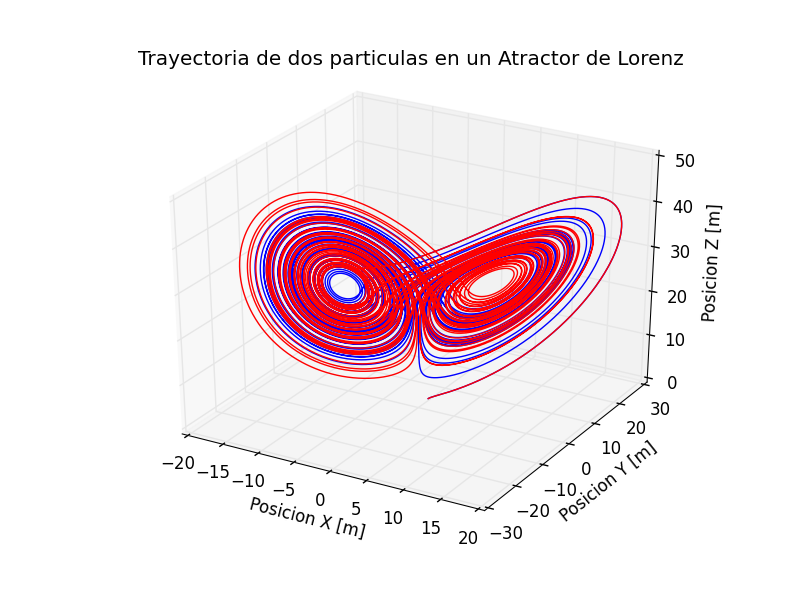
\includegraphics[scale=0.6]{images/atractor_de_lorenz.png}
  \label{}
  \caption{Trayectoria de dos part\'iculas en el Atractor de Lorenz. La curva azul corresponde a la part\'icula 1 y la roja a la part\'icula 2.}
\end{figure}

\subsection{Conclusiones P2}

En este caso se observa como una peque\~na desviaci\'on en las condiciones iniciales genera trayectorias distintas donde se ve que se alcanzan diferencias de hasta 3 \'ordenes de magnitud respecto a la desviaci\'on original (la diferencia inicial de un cent\'imetro llega a alcanzar cerca de diez metros en uno de los m\'aximos). Esto es caracter\'istico de los sistemas ca\'oticos, donde peque\~nas variaciones en las condiciones iniciales pueden generar sistemas radicalmente distintos.

Desde el punto de vista de la implementaci\'on, se observa que la clase escrita para este problema utiliza muchas funciones replicadas directamente desde la soluci\'on del P1. Debido a ello se vuelve interesante el mejorar el uso de la herencia para futuros programas similares, lo que permitir\'a ahorrar c\'odigo al facilitar la reutilizaci\\on. En particular para este caso, cualquier programa de c\'alculo de trayectorias debiese tener, en general, un tratamiento similar al de las soluciones desarrolladas.  

\end{document}
